\documentclass{sigchi-ext}

\usepackage[T1]{fontenc}
\usepackage{textcomp}
\usepackage[scaled=.92]{helvet} % for proper fonts
\usepackage{graphicx} % for EPS use the graphics package instead
\usepackage{balance}  % for useful for balancing the last columns
\usepackage{booktabs} % for pretty table rules
\usepackage{ccicons}  % for Creative Commons citation icons
\usepackage{ragged2e} % for tighter hyphenation
\usepackage[utf8]{inputenc} 

\def\plaintitle{SIGCHI Extended Abstracts Sample File: Note Initial
  Caps} \def\plainauthor{First Author, Second Author}
\def\emptyauthor{}
\def\plainkeywords{Neurodevelopmental Disorders; children; virtual reality; learning; play; alimentation; autonomy; food pyramid.}
\def\plaingeneralterms{Documentation, Standardization}

\title{GEA - a VR Game for Nutrition Education for Children with Neurodevelopmental Disorders}

\numberofauthors{2}
% Notice how author names are alternately typesetted to appear ordered
% in 2-column format; i.e., the first 4 autors on the first column and
% the other 4 auhors on the second column. Actually, it's up to you to
% strictly adhere to this author notation.
\author{%
  \alignauthor{%
    \textbf{Federica Blanco}\\
    \affaddr{Politecnico di Milano} \\
    \email{federica.blanco@mail.polimi.it} }\alignauthor{%
    %\textbf{Fifth Author}\\
    %\affaddr{YetAuthorCo, Inc.}\\
    %\affaddr{Authortown, BC V6M 22P Canada}\\
    %\email{author5@anotherco.com} } \vfil \alignauthor{%
    \textbf{Giulia Pennati}\\
    \affaddr{Politecnico di Milano}\\
    \email{giulia1.pennati@mail.polimi.it} }%\alignauthor{%
    %\textbf{Sixth Author}\\
    %\affaddr{Universit\'e de Auteur-Sud}\\
    %\affaddr{40222 Auteur France}\\
    %\email{author6@author.fr} } \vfil \alignauthor{%
    %\textbf{Third Author}\\
    %\textbf{Fourth Author}\\    
    %\affaddr{L\={e}khaka Interaction Labs}\\
    %\affaddr{Bengaluru 560 080, India}\\
    %\email{author3@anotherco.com} \\
    %\email{author4@hchi.anotherco.com} }\alignauthor{%
    %\textbf{Seventh Author}\\
    %\affaddr{Department of Skrywer}\\
    %\affaddr{University of Umbhali}\\
    %\affaddr{Cape Town, South Africa}\\
    %\email{author7@umbhaliu.ac.za} } }
    }

\definecolor{linkColor}{RGB}{6,125,233}
\hypersetup{%
  pdftitle={\plaintitle},
%  pdfauthor={\plainauthor},
  pdfauthor={\emptyauthor},
  pdfkeywords={\plainkeywords},
  bookmarksnumbered,
  pdfstartview={FitH},
  colorlinks,
  citecolor=black,
  filecolor=black,
  linkcolor=black,
  urlcolor=linkColor,
  breaklinks=true,
}

% \reversemarginpar%

\begin{document}

%% For the camera ready, use the commands provided by the ACM in the Permission Release Form.
%\CopyrightYear{2007}
%\setcopyright{rightsretained}
%\conferenceinfo{WOODSTOCK}{'97 El Paso, Texas USA}
%\isbn{0-12345-67-8/90/01}
%\doi{http://dx.doi.org/10.1145/2858036.2858119}
%% Then override the default copyright message with the \acmcopyright command.
%\copyrightinfo{\acmcopyright}

\maketitle

\RaggedRight{} 


\begin{abstract}
  	This document describes the design of GEA, a web application for children
with NeuroDevelopmental Disorder that has been developed in cooperation
with a team of therapists and children themselves. GEA wants to achieve the
objective of teaching the nutrition education through a virtual reality game
focused on food pyramid, healthy food and good alimentation avoiding waste
of real food. It is developed keeping in mind the real laboratory that children
do in the specialized center so we reproduce a smart and confortable space in
witch they can play the three different games proposed to them. It is also
possible to choose a level of difficulty to make a personalization based on
child capacities. GEA has also a functionality that replicates the smartphone
screen on a pc screen in such a way that the therapist can see what the child
is doing so he can explain all the dubts or help if there are some difficulties.
\end{abstract}

\keywords{\plainkeywords}

\category{H.5.1}{Information interfaces and presentation}{Multimedia Information Systems}
\category{H.5.2}{Information interfaces and presentation}{User Interfaces}
\category{K.4.2}{Computers and society}{Social Issues}



\section{Introduction}
\marginpar{
  \vspace{50pt} 
    \begin{minipage}{0.925\marginparwidth}
  	  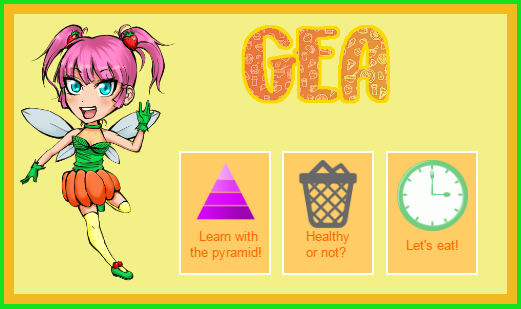
\includegraphics[width=\marginparwidth, height=90px]{figures/Game.png}
  	  \captionof{figure}{GEA home page}
      \label{fig:home page}
      \vspace{30pt}
      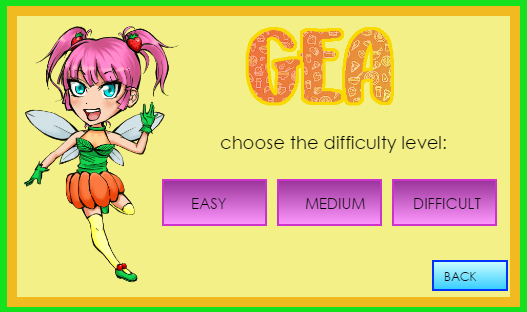
\includegraphics[width=\marginparwidth, height=90px]{figures/Level.png}
  	  \captionof{figure}{GEA levels of difficulty }
      \label{fig:levels}
    \end{minipage}}
NeuroDevelopmental Disorder, NDD, is an umbrela term for a group of disabilities that are caused by a disfunction of a part of the brain or of the nervous system and show their symptoms in the children's physical and psychological development \cite{rif1}. Among the most common diseases we find Autism Spectrum Disorder, ASD, Attention Deficit and Hyperactivity Disorder, ADHD, and Down syndrome \cite{rif2}. Children who suffer from these syndromes need help in developing cognitive abilities such as attention and language, social skills such as the ability to relate to others and personal and domestic autonomy skills.\\
\medskip
 Virtual Reality is nowadays easy to access because it requires the use of a smartphone, owned by the majority of the population, and a VR viewer easily available at low cost; moreover, this technology is much improved so that there are no more problems of feeling sick or difficulty in focusing like in the past \cite{rif6}. The great benefits of using Virtual Reality in an educational and rehabilitation context are now recognized worldwide and tested through various comparative tests between rehabilitation with the use of new technologies and rehabilitation with the use of classical methods \cite{rif3}, \cite{rif4}, \cite{rif5}. The interest in Virtual Reality is so increased also in the field of NDD \cite{rif7}, \cite{rif8}. \\
\medskip
  Our project focuses precisely on this aspect and on the propensity of children to want to have an experience with instruments such as viewers because they are fascinating and attractive. GEA aims to help children with the use of virtual reality to develop their own and domestic autonomy in the field of nutrition, of great importance nowadays as demonstrated during the recent Expo held in Milan \cite{rif11}. Thanks to this game the children will train the memory to remember the different levels of the food pyramid, they will learn to recognize the healthy foods from the so-called "junk foods" and will understand how to combine a meal of the day with a dish and vice versa.


    
\section{Approach}
Our tool is named GEA, Food Education Game, that is in italian Gioco Educazione Alimentare and has been co-designed with NDD specialists from a local therapeutic center. They asked us to transform the feeding laboratory they propose to children once a week with the presence of a specialist in an interactive game.\\
\medskip
 This virtualization has many benefits as the viewer helps to stimulate attention and concentration without any kind of distraction due to external agents. We decided to use virtual reality also because of the ease of use of the instrumentation, as it requires little knowledge of the technology, and for the possibility of being able to reproduce the real environment of the therapy in order to have easy familiarization with the game. The smartphone set inside the VR visor displays the visual contents, splitting them into two near-identical bi-dimensional images, and the interaction is achieved through focus. The user can navigate in the virtual world by rotating his head, which will consequently rotate the virtual scene projected in the display that is a room with some kitchen stuff.\\
\medskip
  The effectiveness of learning by playing also lies in the ability to personalize the session based on the abilities of the individual user: for this reason, three different levels of difficulty have been inserted, among which the therapist can decide knowing the patient's knowledge. To increase personalization we have also decided to divide GEA into three mini-games as we have been told that each user has more difficulty learning one concept than another, so that in this case the therapist will decide which one experience to make the patient present at that time feel. Finally we opted for this implementation as it makes it possible to continue learning in complete autonomy when you are in any place and at any time of the day.


\section{GEA: Requirements}
The requirements for GEA were collected through meetings with psychologists and experts in the field of neurological disorders and who propose this feeding laboratory activity to their patients. A meeting was also held with all the young people present in the local therapeutic center to discuss with them the idea behind GEA and to know directly from them what they usually do, how they do it, the greatest difficulties they encounter and what they would like expect from this application.
\begin{enumerate}
\item \textit{Requirement 1: Customization}\\
      The therapist must be able to set a level of difficulty in the game based on the child's skills so 		  as to start from his level of knowledge and then gradually increase.
\item \textit{Requirement 2: Inherent contents}\\
	  The contents of the game must be inherent and reflect those kept during the workshop. For this 			  reason the three mini-games will be based on the food pyramid, on the recognition of healthy foods 		  and on the ability to combine dishes and meal of the day.
\item \textit{Requirement 3: Attention to the graphics}\\
	  Because of the various disabilities possessed by users, the game does not have to present particular 	  colors too cold or animations too abrupt or flashing as they could trigger reactions that would ruin 	  the therapy.
\item \textit{Requirement 4: Graphic explanations}\\
	  Users of GEA range in a gap of age and disability such that there is the possibility that not 			  everyone can read, for this reason we need visual explanations about the goal of the game and how to 	  do it.
\item \textit{Requirement 5: The therapist must see}\\
	  the therapists need to have always under control what the child is doing during the game experience 		  to know where they are improving and where they still find difficulties and to be able to follow the 	  therapy by providing the necessary explanations.
\end{enumerate}

\section{GEA: Design}
Starting from the above requirements GEA is designed like this: at the start of the application the main page is shown in which there is the possibility for the therapist to choose between three games, as shown in Figure \ref{fig:home page}: "Learn with the pyramid!", "Healthy or not?" and "Let's eat!"; the choice will be made via touchscreen on the smartphone. \\
After that will appear the screen shown in Figure \ref{fig:levels} in order to be able to make, always by the expert, the choice for the level of difficulty desired between: easy, medium and difficult. The difficulty does not lie in the way the game is played or in its objective but in the type of food shown. In the screen there is also a button called "back" to give the possibility to come back if there was a wrong choice in the type of game.\\
After the level of difficulty is selected the game starts.\\
The environment turns out to be identical for all three games in order to be able to follow the real setting of the therapy: there is a room with a table, a fridge, a window, a door, a sofa and a kitchen in order to make the space confortable but also inherent with alimentation. In front of the user will appear a short explanation and a play button.\\
\medskip
\begin{figure*}
 \begin{minipage}[c]{\columnwidth}
   \centering
   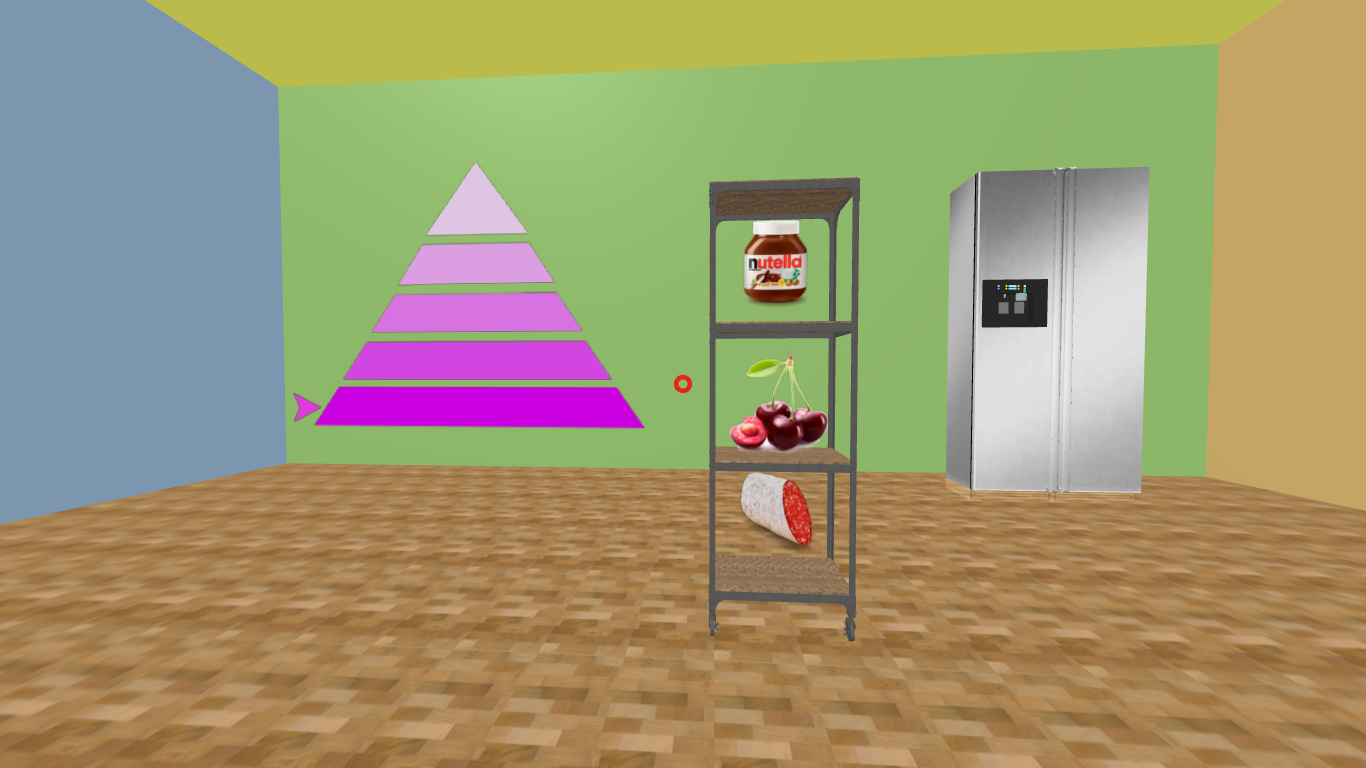
\includegraphics[width=8cm]{figures/Pyramid1.png}
   \caption{"Learn with the pyramid"}
   \label{fig:Pyramid}
 \end{minipage}
 \ \hspace{2mm} \hspace{3mm} \
 \begin{minipage}[c]{\columnwidth}
  \centering
   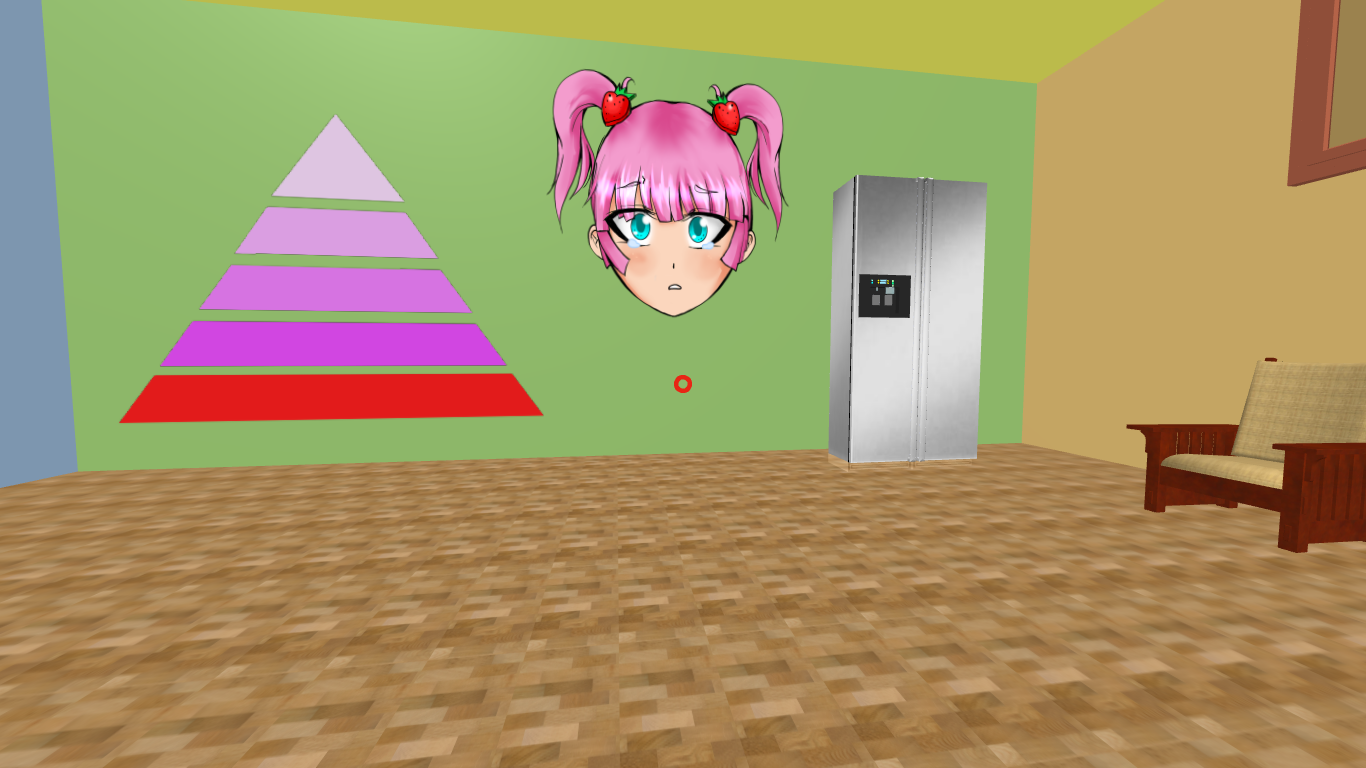
\includegraphics[width=8cm]{figures/Wrong.png}
   \caption{Wrong answer}
   \label{fig:wrong}
 \end{minipage}
\end{figure*}
\textit{\textbf{"Lear with the pyramid!"}}: this game is proposed in order to learn which food goes in which level of the pyramid. As shown in Figure \ref{fig:Pyramid}, on the screen disapear the table and appear on the wall a pyramid divided into five levels, a pointer that indicates which level you have to complete and a mobile with three options. The red circle is the pointer and you have to point to one of the food for a time interval to give the answer, this is to avoid that someone gives an answer when he is looking around. After an answer is given a feedback appears, like in Figure \ref{fig:wrong}, with a sad mascotte if it is wrong and the correspondent level coloured red or an happy mascotte if it is correct and the level coloured green.\\
\medskip
\marginpar{
  \vspace{-90pt} 
    \begin{minipage}{0.925\marginparwidth}
  	  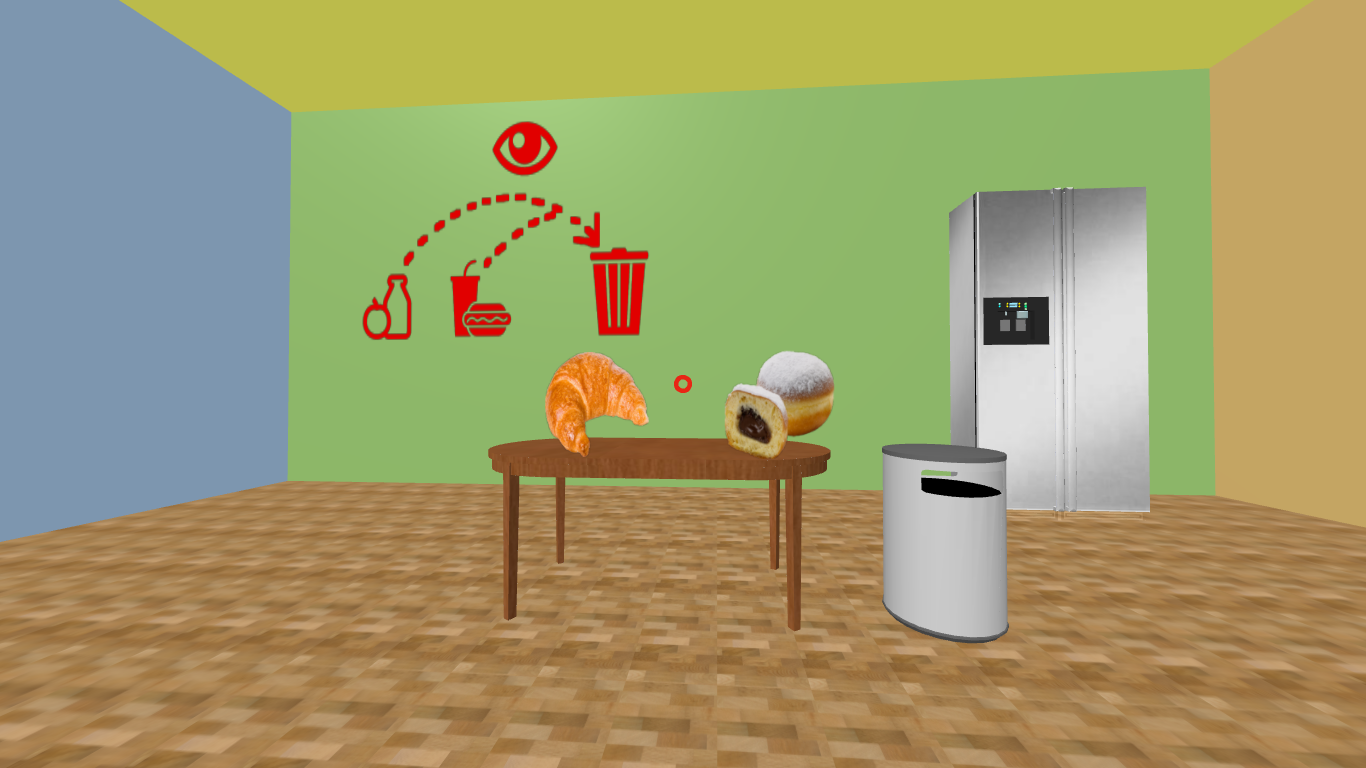
\includegraphics[width=\marginparwidth, height=90px]{figures/Healthy.png}
  	  \captionof{figure}{"Healthy or not?"}
      \label{fig:healthy}
      \vspace{30pt}
      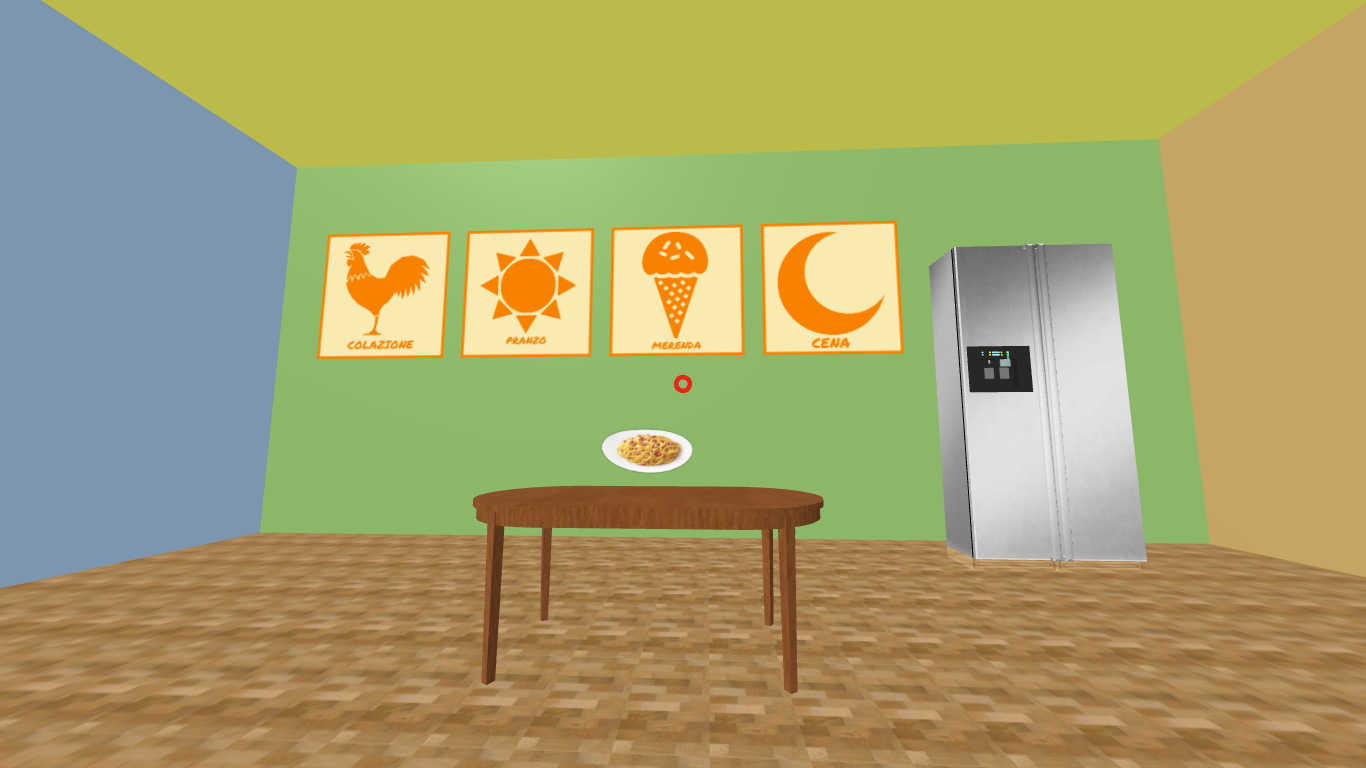
\includegraphics[width=\marginparwidth, height=90px]{figures/Eat.png}
  	  \captionof{figure}{"Let's eat!"}
      \label{fig:eat}
    \end{minipage}}
\textit{\textbf{"Healthy or not?"}}: this game is proposed in order to learn if a food is healthy or not. As shown in Figure \ref{fig:healthy}, on the screen appear on the table two dishes, a bin and a visual explanation: with the eyes you have to move and throw in the bin the junk food. There are three sessions of this game and after each answer there is a feedback like before.\\
\medskip
\textit{\textbf{"Let's eat!"}}: this game is proposed in order to learn if in a meal of the day i can or not eat a specific dish. This game was explicitly required by young people who spoke with us because they have some difficulties to understand when they can eat something or they can not. As shown in Figure \ref{fig:eat} there are all the four meal of the day and a dish: the objective is to select the correct meal/s in which i can eat it. This game is proposed also in the vice versa mode. It is composed by three sessions and after each answer there is a feedback.\\
\medskip
At the end of all the sessions of the mini-games is shown the totalized points and the application comes back automatically to the home page.\\
\medskip
The therapist can view the entire session of play performed by the child thanks to the use of Google Chromecast which allows the replication of the smartphone screen on the PC on which it is installed \cite{rif9}.


\section{GEA: Implementation}
GEA is developed as web applications, which ensures a high degree of portability of all our technology on any platform. We used standard web languages: HTML, JavaScript (for the client side) and PHP (for the server side) and a public software library, A-Frame, that is an open-source web framework for creating 3D and virtual reality applications with JavaScript and HTML \cite{rif10}.

\section{Conclusions and future work}
Our solution turns out to be a good solution for various reasons such as:
\begin{itemize}
\item Virtual reality allows you to have a large database with presence of all possible foods without having to use real food that would be then wasted;
\item GEA turns out to be a compact solution because it only needs a smartphone, now owned by the majority
part of the population, and a VR viewer, available for purchase minimum, so easily transportable;
\item GEA, due to the easy availability of the technology used, allows to the child to be able to continue his education in the food field even in complete autonomy at home without having to wait for go to the center on the day dedicated to the feeding laboratory;
\item Thanks to the presence of a nice and colorful graphics this application allows you to have a fun experience motivating children in learning by playing.
\end{itemize}

As emerged during the various interviews with the therapists, a possible development future in the short term of GEA will result in the introduction of the possibility of the psychologist's interaction during the game: we will then implement one function to pause the game on the smartphone inside th viewer using the PC so that the children can have the necessary explanations in case of doubt or the expert can ask the reasons for that they pushed to a certain choice rather than another and to understand so better what the subjective difficulties are.\\

A further development will take place in the field of allergies: the possibility is assumed to be able to add a game that allows children to identify which ones allergens are present in various foods as essential nowadays be able to understand what to eat or not in case of symilar problems. This addition also emerged during the meetings and was requested from intolerant kids who want to learn how to manage alone this problematic.

%\section{References Format}
\renewcommand\refname{ciao}
\begin{thebibliography}{100}
\bibitem{rif1} EPA, "United States Environmental Protection Agency". America's Children and the Environment | Third Edition, Updated October 2015. 
\url{https://www.epa.gov/sites/production/files/2015-10/documents/ace3_neurodevelopmental.pdf}
\bibitem{rif2} American Psychiatric Association, 2013. Diagnostic and statistical manual of mental disorders (DSM-5®). American Psychiatric Pub. 
\bibitem{rif3} Trevor Hall, Lin Lin, Fabrizia Mantovani, Nigel Newbutt, Thomas D. Parsons, Sarah Parsons, Giuseppe Riva, Eva Venturini, . "Virtual Reality in Pediatric Psychology"
\url{http://pediatrics.aappublications.org/content/pediatrics/140/Supplement_2/S86.full.pdf}
\bibitem{rif4} Denise Reid, Michelle Wang. "Virtual Reality in Pediatric Neurorehabilitation:Attention Deficit Hyperactivity Disorder, Autism and Cerebral Palsy"
\url{https://www.karger.com/Article/Pdf/320847} 
\bibitem{rif5} "Effectiveness of virtual reality using Wii gaming technology in children with Down syndrome", Research in Developmental Disabilities Volume 32, Issue 1, January–February 2011, Pages 312-321
\bibitem{rif6} Strickland, D. C., Marcus, L. M., Mesibov, G. B., Hogan, K. 1996. Brief report: Two case studies using virtual reality as a learning tool for autistic children. Journal of Autism and Developmental Disorders, 26(6), 651–659
\bibitem{rif7} Franca Garzotto, Mirko Gelsomini, and Daniele Occhiuto. 2016 (Conference Paper). Wildcard: A Wearable Virtual Reality Storytelling Tool for Children with Intellectual Developmental Disability Annual International Conference of the IEEE Engineering in Medicine and Biology Society (EMBC’16)
\bibitem{rif8} Mirko Gelsomini. 2016. Best Student Research Paper Award: An Affordable Virtual Reality Learning Framework for Children with Neuro-Developmental Disorder. InProceedings of the 18th International ACM SIGACCESS Conference on Computers and Accessibility(ASSETS '16). ACM, New York, NY,USA, 343-344. DOI: \url{https://doi.org/10.1145/2982142.2982143}
\bibitem{rif9} Google Chromecast. \url{https://chromecast.com}
\bibitem{rif10} A-Frame. \url{https://aframe.io/}
\bibitem{rif11} EXPO 2015, Milan. \url{www.expo2015.org/}
\end{thebibliography}

\balance{} 
\bibliographystyle{SIGCHI-Reference-Format}
%\bibliography{sample}
\end{document}

%%% Local Variables:
%%% mode: latex
%%% TeX-master: t
%%% End:
